\documentclass{aion}

% ------------------------------------------------------------
% Metadata for this paper
% ------------------------------------------------------------
\renewcommand{\papertitle}{WARP Graphs: Emergent Dynamics from Deterministic Rewrite Systems}
\renewcommand{\papernumber}{Paper V}
\renewcommand{\paperdate}{January 2026}
\renewcommand{\paperdoi}{10.5281/zenodo.18146884}

\renewcommand{\paperauthor}{James Ross}
\renewcommand{\paperaffiliation}{Independent Researcher}
\renewcommand{\paperorcid}{0009-0006-0025-7801}

% ------------------------------------------------------------
% Extra packages needed by this paper
% ------------------------------------------------------------
\usepackage{float}
\usepackage{mathtools}  % For \coloneqq
\usepackage{tikz}
\usetikzlibrary{arrows.meta,positioning,decorations.pathreplacing}
\usetikzlibrary{3d}
\usetikzlibrary{backgrounds}

\input{macros}

% ------------------------------------------------------------
% Notation shortcuts (guarded to avoid clashes)
% ------------------------------------------------------------
\ifdefined\WCat\else\newcommand{\WCat}{\mathcal{W}}\fi
\ifdefined\AION\else\newcommand{\AION}{AI$\Omega$N}\fi
\ifdefined\COMPUTER\else\newcommand{\COMPUTER}{C$\Omega$MPUTER}\fi
\ifdefined\sectionbreak\else\newcommand{\sectionbreak}{\clearpage}\fi
\ifdefined\cref\else\newcommand{\cref}{\ref}\fi

% Rewrite / evolution notation (if not already provided by macros.tex)
\ifdefined\Rewrite\else\newcommand{\Rewrite}{\Rightarrow}\fi
\ifdefined\Apply\else\newcommand{\Apply}{\operatorname{Apply}}\fi
\ifdefined\Recon\else\newcommand{\Recon}{\operatorname{Recon}}\fi

% Give hyperref unique anchors for figures to silence duplicate-destination warnings
\makeatletter
\renewcommand{\theHfigure}{\thesection.\arabic{figure}}
\makeatother

\widowpenalty=10000
\clubpenalty=10000
\displaywidowpenalty=10000
\raggedbottom

\begin{document}

\AIONTitlePage

\cleardoublepage
\thispagestyle{empty}

\begin{center}
{\small
\vspace*{\fill}

\textcopyright~2026 James Ross\\[0.75em]

This work is licensed under the\\
\textbf{Creative Commons Attribution 4.0 International License (CC BY 4.0).}\\[1em]

You are free to:
\begin{itemize}[leftmargin=2em]
  \item \textbf{Share} — copy and redistribute the material in any medium or format
  \item \textbf{Adapt} — remix, transform, and build upon the material for any purpose
\end{itemize}

Under the following terms:
\begin{itemize}[leftmargin=2em]
  \item \textbf{Attribution} — You must give appropriate credit, provide a link to the license,\\
        and indicate if changes were made. You may not imply endorsement by the author.
\end{itemize}

For the full legal code of the license, see:\\[0.25em]
\url{https://creativecommons.org/licenses/by/4.0/}

\vspace*{\fill}
}
\end{center}

\cleardoublepage

\begin{abstract}
This paper introduces the dynamical principle of the \AION{} framework. While Papers I--IV~\cite{ross_paper_i, ross_paper_ii, ross_paper_iii, ross_paper_iv} establish the kinematics, measure, and observer geometry of deterministic rewrite systems, they do not specify the mechanism by which a realised worldline is selected from the bundle of admissible histories. We address this gap by equipping rewrite histories with a local action functional and associated complex amplitude measure, from which probabilistic behaviour and effective dynamics emerge through observer projection.

We formalise observers as mappings over bundles of worldlines and derive observed probabilities from interference between observationally indistinguishable histories. This yields quantum-like interference under coarse-grained observation and classical determinism in the presence of full provenance. We prove that the induced evolution is unitary when the rewrite system satisfies local reversibility, action antisymmetry, and branch conservation, combined with complete observer partitions. The resulting dynamics admits a principled notion of stationary action over rewrite paths.

Finally, we show that, under appropriate locality and scaling assumptions, the discrete dynamics admits a continuum approximation equivalent to a Schrödinger-type evolution, establishing a Quantum Cellular Automaton interpretation of the \AION{} system. These results complete the foundational account of \AION{} by providing an explicit dynamical law compatible with its rewrite-theoretic and observer-theoretic structure.
\end{abstract}

\clearpage
\tableofcontents
\clearpage

\section{Introduction}\label{sec:intro}

Paper IV~\cite{ross_paper_iv} completed the geometric and observer-theoretic foundations of the \AION{} Foundations Series. At that stage, the framework specified the structure of admissible histories, the role of observers, and the geometry induced by rulial distance, but it did not specify a dynamical principle governing how realised worldlines arise from this structure. This omission was substantive, not merely expository; an explicit account of dynamics is required to complete the foundational description.

This paper introduces such a dynamical principle. We equip deterministic rewrite systems with a local action functional and associated complex amplitude measure defined over rewrite histories. This construction allows probabilistic behaviour, interference, and effective unitary evolution to emerge from deterministic graph rewriting through observer projection, without assuming intrinsic randomness or continuum postulates.

\subsection{Motivation and Position in the Series}

In physics, the distinction between kinematics---the description of admissible motion---and dynamics---the principles governing realised motion---is fundamental. Papers I--IV of the \AION{} Foundations Series~\cite{ross_paper_i, ross_paper_ii, ross_paper_iii, ross_paper_iv} establish the kinematic foundation of the system: the rewrite rules, the structure of histories, the measurement model, and the geometry of observers. What remains unspecified is the mechanism by which a particular worldline is selected, or appears to be selected, from the bundle of admissible histories.

The purpose of this paper is to close this gap. Rather than introducing an external scheduler or stochastic choice rule, we show that dynamics can be derived internally by assigning actions and amplitudes to rewrite histories and analysing their behaviour under observer coarse-graining. In this sense, the present work completes the transition from a purely kinematic framework to a dynamical one.

\subsection{Contributions}

The contributions of this paper are as follows:
\begin{itemize}
    \item \textbf{Rewrite Histories with Amplitudes.} We formalise bundles of rewrite paths (worldlines) and equip them with a local action functional and complex amplitude measure, enabling interference between deterministic histories.
    \item \textbf{Observer-Induced Probabilities.} We refine the observer model of Paper IV as a mapping over worldline bundles and derive observed probabilities from amplitude interference between observationally indistinguishable histories, recovering both quantum-like and classical limits.
    \item \textbf{Emergent Unitarity.} We prove that unitary evolution is not assumed but emerges from structural properties of the rewrite system—specifically local reversibility, action antisymmetry, and branch conservation, combined with complete observer partitions (Theorem~1).
    \item \textbf{Graph-Theoretic Action Principle.} We construct a rewrite-local generator grounded in DPO rule structure, yielding a principled notion of stationary action over rewrite paths that balances structural change against contextual complexity.
    \item \textbf{Continuum Approximation.} We show that, under appropriate locality and scaling assumptions, the discrete dynamics admits a Quantum Cellular Automaton interpretation and yields a Schrödinger-type evolution equation as an effective limit.
\end{itemize}

\subsection{Scope and Roadmap}

This paper is concerned exclusively with the theoretical dynamics of the \AION{} framework. We do not address implementation-specific scheduling policies, optimisation strategies, or system architecture, which are deferred to subsequent work. The goal here is to establish the minimal dynamical principles compatible with the rewrite-theoretic and observer-theoretic foundations already developed.

The remainder of the paper is organised as follows. Section~\ref{sec:states} formalises the state space and rewrite histories. Section~\ref{sec:action} introduces the action functional and amplitude measure. Section~\ref{sec:unitarity} analyses the emergence of unitary evolution. Section~\ref{sec:continuum} examines the continuum approximation and effective Schrödinger dynamics. We conclude with a discussion of implications and limitations.

\subsection*{Related Lineage}

The ideas developed in this paper draw on several established lines of research. Multiway rewriting systems and rulial geometry build on concepts introduced in Wolfram's work on multiway systems~\cite{wolfram_nks} and the Wolfram Physics Project~\cite{wolfram_physics_project}. The use of action-weighted path summation parallels Feynman's path-integral formulation of quantum mechanics~\cite{feynman_space_time}. The formal treatment of rewriting relies on the Double Pushout framework developed by Ehrig and collaborators~\cite{ehrig_graph_transformations}. Finally, the connection between reversibility and conservation draws on foundational results in reversible computation due to Landauer~\cite{landauer_irreversibility} and Bennett~\cite{bennett_logical_reversibility}. The present work differs in that it integrates these strands into a single deterministic rewrite framework in which unitarity and quantum structure are derived rather than postulated.

\section{State Space and Rewrite Histories}
\label{sec:states}

We begin by formalising the kinematic foundation over which the dynamics introduced in this paper will act. This construction builds directly on the rewrite-theoretic foundations established in Papers I–II~\cite{ross_paper_i, ross_paper_ii} and the observer-theoretic framework of Paper IV~\cite{ross_paper_iv}.

\subsection{Structural State Space}

Let $\mathcal{U}$ denote the set of all admissible \WARP{} graph topologies consistent with the type signatures and structural constraints defined in Papers I–II~\cite{ross_paper_i, ross_paper_ii}. Elements of $\mathcal{U}$ are considered up to isomorphism and represent distinct, fully specified structural configurations of the system.

At this stage, states in $\mathcal{U}$ are classical objects: no superposition or probabilistic structure is assumed. The purpose of the present paper is precisely to explain how such structures acquire effective dynamical and probabilistic behaviour.

\subsection{Rewrite Histories and Worldlines}

Let $\mathfrak{R}$ be a fixed set of Double Pushout (DPO) rewrite rules acting on $\mathcal{U}$. A \textit{rewrite history}, or \textit{worldline}, is defined as a finite sequence
\[
\gamma = \bigl(G_0 \xrightarrow{r_1} G_1 \xrightarrow{r_2} \cdots \xrightarrow{r_N} G_N\bigr),
\]
where $G_k \in \mathcal{U}$ and each transition corresponds to a valid application of a rule $r_k \in \mathfrak{R}$.

For a fixed initial state $G_0$, the set of all admissible rewrite histories forms the \textit{multiway bundle} $\Omega(G_0)$. This bundle carries a natural causal partial order inherited from the dependency relations between rewrite events, yielding the multiway graph structure analysed in Paper IV~\cite{ross_paper_iv}.

Importantly, no preference or selection principle is assumed at this level; all admissible histories coexist as elements of $\Omega(G_0)$.

\subsection{Observers and Indistinguishability}

\begin{figure}[htb]
  \centering
  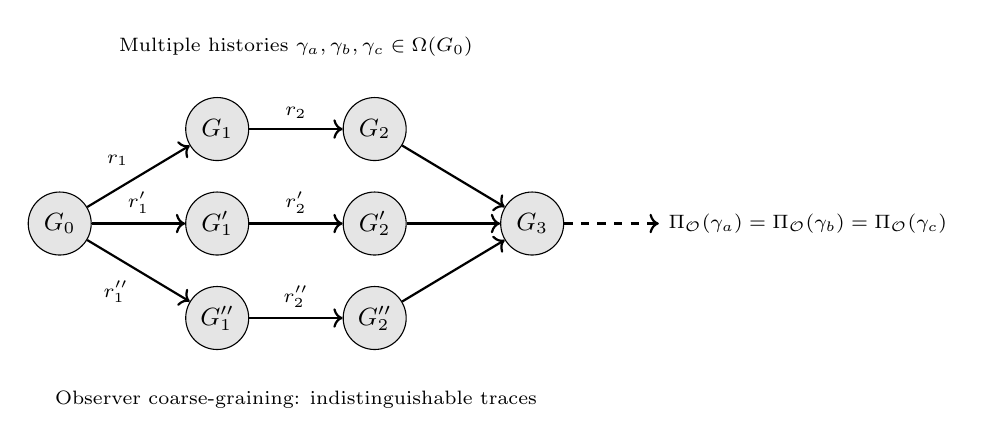
\begin{tikzpicture}[
    font=\small\sffamily,
    state/.style={circle, draw, fill=gray!20, minimum size=8mm, inner sep=0pt},
    history/.style={->, thick},
    observation/.style={->, thick, dashed}
  ]

  % Initial state
  \node[state] (u0) at (0,0) {$G_0$};

  % Multiple rewrite paths
  \node[state] (u1a) at (2,1.2) {$G_1$};
  \node[state] (u1b) at (2,0) {$G_1'$};
  \node[state] (u1c) at (2,-1.2) {$G_1''$};

  \node[state] (u2a) at (4,1.2) {$G_2$};
  \node[state] (u2b) at (4,0) {$G_2'$};
  \node[state] (u2c) at (4,-1.2) {$G_2''$};

  % Final convergence
  \node[state] (u3) at (6,0) {$G_3$};

  % Rewrite histories (multiple paths)
  \draw[history] (u0) -- (u1a) node[midway, above left] {\scriptsize $r_1$};
  \draw[history] (u0) -- (u1b) node[midway, above] {\scriptsize $r_1'$};
  \draw[history] (u0) -- (u1c) node[midway, below left] {\scriptsize $r_1''$};

  \draw[history] (u1a) -- (u2a) node[midway, above] {\scriptsize $r_2$};
  \draw[history] (u1b) -- (u2b) node[midway, above] {\scriptsize $r_2'$};
  \draw[history] (u1c) -- (u2c) node[midway, above] {\scriptsize $r_2''$};

  \draw[history] (u2a) -- (u3);
  \draw[history] (u2b) -- (u3);
  \draw[history] (u2c) -- (u3);

  % Observer projection (coarse-graining)
  \node[align=center, font=\scriptsize, above] at (3, 2.0) {Multiple histories $\gamma_a, \gamma_b, \gamma_c \in \Omega(G_0)$};

  % Observational trace (single perceived path)
  \node (obs) at (9.5,0) {\scriptsize $\Pi_{\mathcal{O}}(\gamma_a) = \Pi_{\mathcal{O}}(\gamma_b) = \Pi_{\mathcal{O}}(\gamma_c)$};
  \draw[observation] (u3) -- (obs.west);

  \node[align=center, font=\scriptsize, below] at (3, -2.0) {Observer coarse-graining: indistinguishable traces};
\end{tikzpicture}

  \caption{\textbf{Observer coarse-graining:} Multiple rewrite histories mapped to a single observational trace.}
\end{figure}

Following Paper IV~\cite{ross_paper_iv}, an observer is defined as a coarse-graining map
\[
\Pi_{\mathcal{O}} : \Omega(G_0) \to \mathcal{T},
\]
where $\mathcal{T}$ denotes a space of \textit{observational traces}. Two histories $\gamma_a$ and $\gamma_b$ are \textit{indistinguishable} to observer $\mathcal{O}$ if
\[
\Pi_{\mathcal{O}}(\gamma_a) = \Pi_{\mathcal{O}}(\gamma_b).
\]

This induces a partition of the multiway bundle into equivalence classes of observationally indistinguishable histories. As shown in Paper IV~\cite{ross_paper_iv}, such coarse-graining is responsible for the emergence of a single perceived temporal ordering. In the present work, these equivalence classes will additionally serve as the domains over which amplitude interference is defined.

We say that an observer projection $\Pi_{\mathcal{O}}$ induces a \textit{complete partition} of $\Omega(G_0)$ if every history $\gamma \in \Omega(G_0)$ is assigned to exactly one equivalence class, and the union of all equivalence classes recovers the entire bundle. Formally, the partition is complete if it satisfies exhaustiveness and disjointness: every history appears in exactly one equivalence class, and no history is discarded or duplicated. A partition is \textit{measure-preserving} if the total amplitude norm is conserved under the coarse-graining operation, i.e.\ no amplitude is lost through the projection.

\begin{definition}[Complete Partition]
\label{def:complete_partition}
An observer projection $\Pi_{\mathcal{O}} : \Omega(G_0) \to \mathcal{T}$ induces a \emph{complete partition} if:
\begin{enumerate}[label=(\roman*)]
    \item \textbf{Surjectivity:} For every $\tau \in \mathcal{T}$, there exists $\gamma \in \Omega(G_0)$ such that $\Pi_{\mathcal{O}}(\gamma) = \tau$.
    \item \textbf{Disjoint fibers:} For distinct $\tau_1, \tau_2 \in \mathcal{T}$,
    $\Pi_{\mathcal{O}}^{-1}(\tau_1) \cap \Pi_{\mathcal{O}}^{-1}(\tau_2) = \emptyset$.
    \item \textbf{Exhaustiveness:} $\Omega(G_0) = \bigsqcup_{\tau \in \mathcal{T}} \Pi_{\mathcal{O}}^{-1}(\tau)$.
\end{enumerate}
The partition is \emph{measure-preserving}~\cite{rudin_real_complex, halmos_measure_theory} if the amplitude measure satisfies
\[
\sum_{\gamma \in \Omega(G_0)} |\phi[\gamma]|^2 = \sum_{\tau \in \mathcal{T}} |\Phi_{\mathcal{O}}(\tau)|^2,
\]
where $\Phi_{\mathcal{O}}(\tau) = \sum_{\gamma \in \Pi_{\mathcal{O}}^{-1}(\tau)} \phi[\gamma]$.
\end{definition}

\subsection{Linearisation as an Observational Construct}

We introduce a linear structure only after defining rewrite histories and observer-induced equivalence classes. For a fixed observer $\mathcal{O}$, we consider the complex vector space generated by the equivalence classes of histories in $\Omega(G_0)$. This linearisation provides a convenient representation for computing interference effects but is not taken to be ontologically fundamental.

In subsequent sections, we equip individual histories with actions and complex amplitudes. The effective state vectors familiar from quantum formalisms will arise as summaries of amplitude distributions over observer-defined equivalence classes, rather than as primitive objects.

\section{The Action Functional and Amplitude Measure}
\label{sec:action}

Having defined the bundle of admissible rewrite histories $\Omega(G_0)$, we now introduce the dynamical principle that distinguishes realised behaviour from mere structural possibility. The central assumption of this paper is that rewrite dynamics are governed by a discrete principle of \textit{stationary action}, defined locally over rewrite events and globally over histories.

\subsection{Local Rewrite Lagrangian}

To each rewrite event $r_k : G_{k-1} \to G_k$, we associate a \textit{discrete Lagrangian} $\mathcal{L}$ capturing the local structural cost of the transition. We define
\[
\mathcal{L}(G_{k-1}, G_k) \coloneqq \mathcal{K}(r_k) - \frac{\mathcal{V}(G_{k-1}) + \mathcal{V}(G_k)}{2},
\]
where the symmetric mean potential is adopted to ensure invariance under time reversal.

The \textit{kinetic term} $\mathcal{K}(r_k)$ quantifies the immediate structural change induced by the rewrite and is measured by the \WARP{} edit distance, i.e.\ the number of primitive graph elements created, destroyed, or relinked by the rule application.

The \textit{potential term} $\mathcal{V}(G_k)$ quantifies the contextual complexity of the resulting state and is defined in terms of its hierarchical depth and recursive density.\footnote{While $\mathcal{V}$ is defined abstractly here to maintain generality, concrete realisations may include subgraph centrality, graph edit distance from a reference state, or computable approximations to Kolmogorov complexity (e.g., Lempel-Ziv complexity~\cite{lempel_ziv_complexity} of the graph's adjacency matrix).} Intuitively, this term penalises rewrites that move the system into structurally rigid or highly constrained configurations.\footnote{Physically, this is analogous to the potential energy of a compressed spring or a particle in a field: the system ``wants'' to evolve toward states of lower structural tension (lower complexity cost). Here, high-complexity states effectively sit higher in the potential well, making them dynamically costly to access without sufficient kinetic input.} In practice, $\mathcal{V}$ may be instantiated using measures such as attachment depth or subgraph description length; no single choice is assumed in this paper.

\paragraph{Concrete Instantiation.} For computational implementation and verification, we adopt the following specific form for $\mathcal{V}$:
\[
\mathcal{V}(G) \coloneqq \alpha \cdot \mathcal{C}_{\mathrm{LZ}}(G) + \beta \cdot \mathrm{diam}(G) + \gamma \cdot \mathcal{E}_{\mathrm{attach}}(G),
\]
where:
\begin{itemize}
    \item $\mathcal{C}_{\mathrm{LZ}}(G)$ is the Lempel-Ziv complexity~\cite{lempel_ziv_complexity} of the adjacency matrix representation of $G$,
    \item $\mathrm{diam}(G)$ is the graph diameter,
    \item $\mathcal{E}_{\mathrm{attach}}(G) = \sum_{v \in V(G)} \mathrm{depth}(v)$ is the total attachment energy, where $\mathrm{depth}(v)$ denotes the provenance depth of vertex $v$ as defined in Paper I~\cite{ross_paper_i}.
\end{itemize}
The coefficients $\alpha, \beta, \gamma \geq 0$ are system-dependent weighting parameters. This choice ensures computability while capturing structural rigidity (via $\mathcal{C}_{\mathrm{LZ}}$), spatial extent (via diameter), and hierarchical constraints (via attachment depth). Alternative formulations using algorithmic information content~\cite{kolmogorov_information} or spectral graph measures may be substituted depending on the application domain.

\subsection{Example: The Action of a Vertex Subdivision}

To ground the abstract definitions of kinetic and potential terms, consider a concrete rewrite rule $r_{\mathrm{sub}}$ implementing a vertex subdivision.

Let the initial state $G_{k-1}$ consist of a single node with a self-loop. The rule $r_{\mathrm{sub}}$ replaces this structure with two nodes connected by a single edge:
\[
G_{k-1} = (\bullet \circlearrowleft) \xrightarrow{r_{\mathrm{sub}}} G_k = (\bullet - \bullet).
\]

We calculate the \textit{kinetic term} $\mathcal{K}(r_{\mathrm{sub}})$ as the graph edit distance required to effect this transition. The operation comprises the deletion of one edge (the self-loop) and the creation of one node and one connecting edge:
\[
\mathcal{K}(r_{\mathrm{sub}}) = 1_{\mathrm{del}} + 1_{\mathrm{node}} + 1_{\mathrm{edge}} = 3.
\]

For the \textit{potential term}, we adopt a toy complexity measure where $\mathcal{V}(G)$ is proportional to the graph diameter. For the initial state $G_{k-1}$ (one node), $\mathcal{V}(G_{k-1}) = 0$. For the resulting state $G_k$ (two connected nodes), $\mathcal{V}(G_k) = 1$.

The \textit{local Lagrangian} for this rewrite step is therefore:
\[
\mathcal{L}(G_{k-1}, G_k) = \mathcal{K}(r_{\mathrm{sub}}) - \frac{\mathcal{V}(G_{k-1}) + \mathcal{V}(G_k)}{2} = 3 - 0.5 = 2.5.
\]

Assuming a unit causal increment $\Delta \tau = 1$, the action contribution for this step is $\mathcal{S} = 2.5$ (in units of structural action). The associated complex amplitude factor contributed to the history is:
\[
\phi_{\mathrm{step}} = \exp\!\left(\frac{2.5i}{\hbar_{\mathfrak{R}}}\right).
\]
This phase factor represents the dynamical ``weight'' of selecting this subdivision path versus purely maintaining the self-loop (which might have $\mathcal{K}=0, \mathcal{V}=0, \mathcal{L}=0$, yielding $\phi=1$). 

\subsection{Action over Rewrite Histories}

The action associated with a rewrite history $\gamma$ is defined as the cumulative contribution of the local Lagrangian along the history:
\[
\mathcal{S}[\gamma] = \sum_{k=1}^{N} \mathcal{L}(G_{k-1}, G_k)\,\Delta \tau_k.
\]
Here, $\Delta \tau_k$ denotes the \textit{causal increment} associated with the $k$th rewrite event, which may be taken to correspond to unit causal depth or event ordering in the multiway graph. Dimensionally, when $\mathcal{L}$ is measured in units of structural change and $\Delta \tau_k$ is dimensionless (representing discrete event count), the action $\mathcal{S}[\gamma]$ inherits the same units as the Lagrangian. The quantity $\hbar_{\mathfrak{R}}$, defined below, serves to render the phase $\mathcal{S}/\hbar_{\mathfrak{R}}$ dimensionless, ensuring consistency in the amplitude assignment. The action thus represents the total structural effort embodied by a particular history.

We say that the action functional satisfies \textit{action antisymmetry} if, for every reversible rewrite history $\gamma$ with corresponding inverse history $\gamma^{-1}$ (obtained by traversing the same sequence of states in reverse using inverse rules), the actions are related by
\[
\mathcal{S}[\gamma^{-1}] = -\mathcal{S}[\gamma].
\]
To ensure this, we define the \textit{causal increment} $\Delta \tau$ as a signed quantity: $\Delta \tau = +1$ for forward evolution and $\Delta \tau = -1$ for retrodiction. Since the kinetic term $\mathcal{K}$ and the symmetric potential term defined in Section~\ref{sec:action} are even under reversal, the sign change in $\Delta \tau$ guarantees that forward and reverse traversals contribute conjugate phases to the amplitude measure. This property is strictly required for microscopic time-reversal symmetry.

\subsection{Amplitude Assignment and Interference}

\begin{figure}[htb]
  \centering
  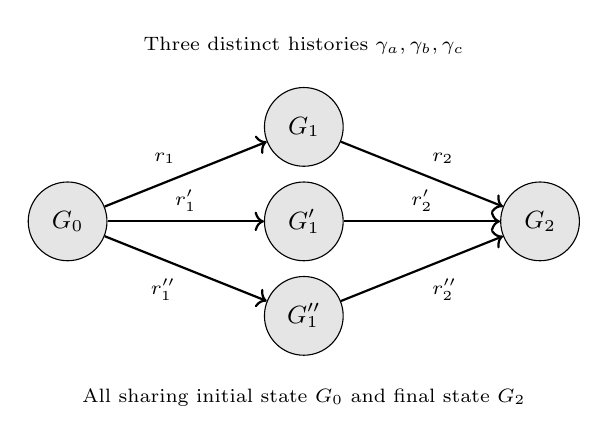
\begin{tikzpicture}[
    font=\small\sffamily,
    state/.style={circle, draw, fill=gray!20, minimum size=10mm, inner sep=0pt},
    history/.style={->, thick}
  ]

  % Initial state G_0
  \node[state] (g0) at (0,0) {$G_0$};

  % Multiple intermediate states
  \node[state] (g1a) at (3,1.2) {$G_1$};
  \node[state] (g1b) at (3,0) {$G_1'$};
  \node[state] (g1c) at (3,-1.2) {$G_1''$};

  % Final state G_2
  \node[state] (g2) at (6,0) {$G_2$};

  % Multiple paths from G_0 to intermediate states
  \draw[history] (g0) -- (g1a) node[midway, above left] {\scriptsize $r_1$};
  \draw[history] (g0) -- (g1b) node[midway, above] {\scriptsize $r_1'$};
  \draw[history] (g0) -- (g1c) node[midway, below left] {\scriptsize $r_1''$};

  % Multiple paths from intermediate states to G_2
  \draw[history] (g1a) -- (g2) node[midway, above right] {\scriptsize $r_2$};
  \draw[history] (g1b) -- (g2) node[midway, above] {\scriptsize $r_2'$};
  \draw[history] (g1c) -- (g2) node[midway, below right] {\scriptsize $r_2''$};

  % Labels for histories
  \node[align=center, font=\scriptsize, above] at (3, 2.0) {Three distinct histories $\gamma_a, \gamma_b, \gamma_c$};
  \node[align=center, font=\scriptsize, below] at (3, -2.0) {All sharing initial state $G_0$ and final state $G_2$};

\end{tikzpicture}

  \caption{\textbf{Multiway interference:} Distinct histories sharing initial and final states ($G_0, G_2$) but diverging locally produce amplitude interference under observer projection.}
\end{figure}

We assign to each history $\gamma \in \Omega(G_0)$ a complex amplitude
\[
\phi[\gamma] \coloneqq \left( \prod_{k=1}^{N} \frac{1}{\sqrt{\operatorname{deg}_{\mathrm{out}}(G_{k-1})}} \right) \exp\!\left(\frac{i}{\hbar_{\mathfrak{R}}}\,\mathcal{S}[\gamma]\right),
\]
where $\operatorname{deg}_{\mathrm{out}}(G)$ denotes the branching degree (number of valid rewrite applications) at state $G$. The normalisation factor ensures that amplitude flux is conserved at branching points, maintaining the $\ell^2$ norm of the superposition state. Here, $\hbar_{\mathfrak{R}}$ is a system-dependent scaling constant setting the resolution at which action differences are dynamically significant. The quantity $\hbar_{\mathfrak{R}}$ has units of action measured in rewrite-steps; in purely structural systems it may be taken to be dimensionless. No probabilistic interpretation is assumed at this stage.

Given an observer $\mathcal{O}$ with projection $\Pi_{\mathcal{O}}$, histories are grouped into equivalence classes $[\gamma]_{\mathcal{O}}$.
(Note that while we treat the observer $\mathcal{O}$ operationally here as an external projection map for mathematical clarity, the wider \AION{} framework models observers as subgraph structures intrinsic to the system. The projection $\Pi_{\mathcal{O}}$ is thus the effective view of the system relative to that internal observer's frame.)

The \textit{effective amplitude} associated with an observational outcome is obtained by summing amplitudes within each class:
\[
\Phi_{\mathcal{O}}([\gamma]) = \sum_{\gamma' \in [\gamma]_{\mathcal{O}}} \phi[\gamma'].
\]
Constructive and destructive interference within this sum govern which outcomes are realised with high probability. In the discrete setting, histories with locally extremal action—where small combinatorial perturbations yield minimal net action variation—contribute coherently, whereas histories with rapidly varying action interfere destructively.

\subsection{Classical and Quantum Limits}

This formulation recovers classical deterministic behaviour in the limit of maximal observational resolution. If an observer $\mathcal{O}_{\mathrm{fine}}$ distinguishes all rewrite events, each equivalence class reduces to a singleton and no interference occurs. The system then appears as a deterministic, branching rewrite process.

\begin{figure}[htb]
  \centering
  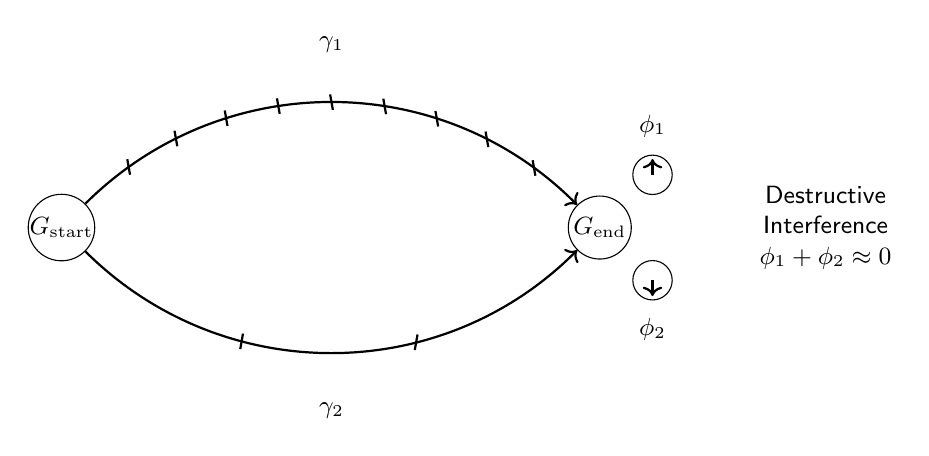
\begin{tikzpicture}[
    scale=1.0,
    node distance=4cm,
    every node/.style={font=\small\sffamily},
    state/.style={circle, draw, minimum size=0.8cm, fill=white, inner sep=0pt},
    phasor/.style={circle, draw, minimum size=0.5cm, inner sep=0pt, fill=white}
]

% Nodes
\node[state] (start) {$G_{\mathrm{start}}$};
\node[state, right=6cm of start] (end) {$G_{\mathrm{end}}$};

% Paths
\draw[->, thick, bend left=45] (start) to node[midway, above=0.5cm] (path1) {$\gamma_1$} (end);
\draw[->, thick, bend right=45] (start) to node[midway, below=0.5cm] (path2) {$\gamma_2$} (end);

% Ticks on path 1 (High Action)
\foreach \t in {0.1, 0.2, ..., 0.9} {
    \path (start) to[bend left=45] coordinate[pos=\t] (m) (end);
    \draw[thick] (m) ++(100:0.1) -- ++(-80:0.2); 
}

% Ticks on path 2 (Low Action)
\foreach \t in {0.33, 0.66} {
    \path (start) to[bend right=45] coordinate[pos=\t] (m) (end);
    \draw[thick] (m) ++(80:0.1) -- ++(-100:0.2);
}

% Phasors at destination
\node[phasor, above right=0.2cm and 0.2cm of end] (p1) {};
\draw[->, thick] (p1.center) -- ++(90:0.2cm); % Up
\node[above=0.1cm of p1] {$\phi_1$};

\node[phasor, below right=0.2cm and 0.2cm of end] (p2) {};
\draw[->, thick] (p2.center) -- ++(270:0.2cm); % Down
\node[below=0.1cm of p2] {$\phi_2$};

% Interference label
\node[right=1.5cm of end, align=center] {Destructive\\Interference\\$\phi_1 + \phi_2 \approx 0$};

\end{tikzpicture}

  \caption{\textbf{Path interference:} Distinct actions $\mathcal{S}_1 \neq \mathcal{S}_2$ for histories reaching $G_{\mathrm{end}}$ create relative phase differences, causing constructive or destructive interference.}
\end{figure}

Conversely, under coarse-grained observation, multiple histories contribute to the same observational trace, and interference effects become observable. Quantum-like probabilistic behaviour thus emerges not from intrinsic randomness, but from the interaction between deterministic rewrite dynamics and coarse-graining by the observer.

The transition between these regimes is governed by the granularity of the observer projection $\Pi_{\mathcal{O}}$. As the observer's resolution decreases, the equivalence classes $[\gamma]_{\mathcal{O}}$ grow larger, admitting more histories per observational trace. The resulting amplitude superposition produces interference patterns characteristic of quantum systems. Conversely, as observation becomes more fine-grained, each equivalence class shrinks towards a singleton, interference is suppressed, and the system exhibits classical, deterministic branching behaviour. This observer-dependent transition provides a natural bridge between quantum and classical regimes without invoking decoherence or measurement collapse as primitive postulates.

\section{Emergent Unitarity and Conservation}
\label{sec:unitarity}

A fundamental requirement for consistent dynamical behaviour is the conservation of total amplitude under evolution. In conventional quantum mechanics, this requirement is enforced axiomatically through unitary time evolution. In the \AION{} framework, we show that unitarity emerges from structural properties of the underlying rewrite system combined with observer completeness.

\subsection{Local Reversibility of Rewrite Rules}

We restrict attention to rewrite systems $\mathfrak{R}$ satisfying \textit{local reversibility}. A Double Pushout (DPO) rule
\[
r = (L \leftarrow K \rightarrow R)
\]
is said to be reversible if there exists a corresponding inverse rule
\[
r^{-1} = (R \leftarrow K \rightarrow L),
\]
such that the composition of $r$ and $r^{-1}$ restores the original graph up to isomorphism.

Local reversibility ensures that the causal graph of rewrite events admits bidirectional traversal at the microscopic level. As a result, rewrite histories form a \textit{flux-conserving network}: no amplitude is created or destroyed by the application of reversible rules.

\subsection{Branch Conservation in the Multiway Bundle}

Let $\Omega(G_0)$ denote the multiway bundle of rewrite histories originating from an initial state $G_0$, equipped with amplitudes $\phi[\gamma]$ as defined in Section~\ref{sec:action}. Prior to any observer projection, amplitude flow through the causal graph is conserved by construction: every rewrite event preserves the total incoming and outgoing amplitude flux.

This conservation is purely structural and does not depend on any probabilistic interpretation. Apparent non-conservation arises only after coarse-graining by an observer.

\begin{figure}[htb]
  \centering
  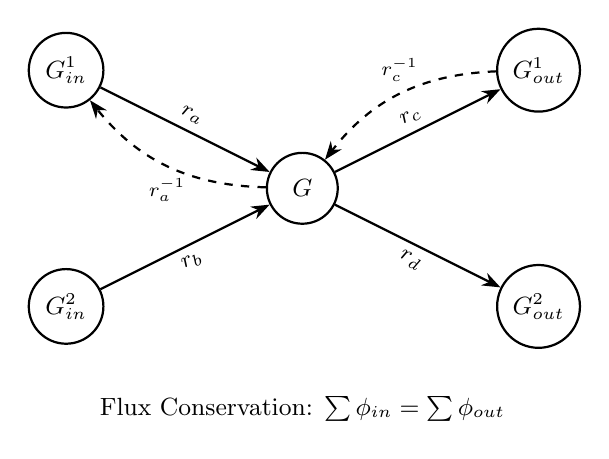
\begin{tikzpicture}[
    scale=1.0,
    node distance=2.5cm,
    font=\small\sffamily,
    state/.style={circle, draw, thick, fill=white, minimum size=0.9cm},
    arrow/.style={->, >=Stealth, thick},
    label/.style={fill=white, inner sep=1pt, font=\footnotesize\sffamily}
  ]

  % Central node
  \node[state] (C) at (0,0) {$G$}; 

  % Incoming nodes - increased vertical spread
  \node[state] (I1) at (-3, 1.5) {$G_{in}^1$}; 
  \node[state] (I2) at (-3, -1.5) {$G_{in}^2$}; 

  % Outgoing nodes - increased vertical spread
  \node[state] (O1) at (3, 1.5) {$G_{out}^1$}; 
  \node[state] (O2) at (3, -1.5) {$G_{out}^2$}; 

  % Edges (Forward) - explicitly positioned labels
  \draw[arrow] (I1) -- node[midway, above=2pt, label, sloped] {$r_a$} (C);
  \draw[arrow] (I2) -- node[midway, below=2pt, label, sloped] {$r_b$} (C);
  \draw[arrow] (C) -- node[midway, above=2pt, label, sloped] {$r_c$} (O1);
  \draw[arrow] (C) -- node[midway, below=2pt, label, sloped] {$r_d$} (O2);

  % Edges (Reverse) - bent further out with tiny font
  \draw[arrow, dashed, bend left=25] (C) to node[midway, below=1pt, font=\scriptsize] {$r_a^{-1}$} (I1);
  \draw[arrow, dashed, bend right=25] (O1) to node[midway, above=1pt, font=\scriptsize] {$r_c^{-1}$} (C);

  % Flux conservation label - moved lower
  \node[align=center, font=\small] at (0, -2.8) {Flux Conservation: $\sum \phi_{in} = \sum \phi_{out}$};

\end{tikzpicture}

  \caption{\textbf{Branch conservation:} Microscopic reversibility ensures flux conservation at every rewrite event.}
\end{figure}

\subsection{Observer Projection and Effective Unitarity}

Given an observer $\mathcal{O}$ with projection $\Pi_{\mathcal{O}}$, histories are grouped into equivalence classes $[\gamma]_{\mathcal{O}}$. The \textit{effective amplitude} associated with an observational outcome is obtained by summing amplitudes within each class:
\[
\Phi_{\mathcal{O}}([\gamma]) = \sum_{\gamma' \in [\gamma]_{\mathcal{O}}} \phi[\gamma'].
\]

If the observer’s partition of $\Omega(G_0)$ is complete and measure-preserving—i.e.\ if all histories are accounted for and no amplitude is discarded—then the induced evolution of the observational amplitude distribution conserves total norm. In this case, the effective dynamics are unitary.

However, if the observer's projection discards or obscures entire classes of histories, apparent non-unitarity arises as informational leakage rather than physical loss.

\paragraph{Verifying Observer Completeness.}
Paper IV~\cite{ross_paper_iv} establishes sufficient conditions for observer completeness via the \emph{provenance partition theorem} (Theorem 3.2 therein). Specifically, if the observer $\mathcal{O}$ is defined by a finite collection of provenance predicates $\{\phi_1, \ldots, \phi_k\}$ forming a Boolean algebra over rewrite events, and if the rulial distance metric $d_{\mathfrak{R}}$ induced by these predicates is complete (i.e., every Cauchy sequence of histories converges), then $\Pi_{\mathcal{O}}$ induces a complete partition of $\Omega(G_0)$. For practical verification, one may construct the quotient graph $\Gamma/\Pi_{\mathcal{O}}$ and verify that its vertex set bijects with $\mathcal{T}$ and its incoming and outgoing degrees match at all vertices. When the observer is defined by coarse-graining over temporal windows or spatial regions, completeness requires that the coarse-graining cells tile the entire history space without gaps or overlaps. In computational implementations, completeness can be checked by ensuring that the sum of pre-image cardinalities equals the total number of histories:
\[
\sum_{\tau \in \mathcal{T}} |\Pi_{\mathcal{O}}^{-1}(\tau)| = |\Omega(G_0)|.
\]

\subsection{Theorem 1: Emergent Unitarity}

We begin with a foundational lemma establishing the connection between causal separation and phase decoherence, which will underpin the orthogonality result.

\begin{lemma}[Phase Decoherence from Causal Separation]
\label{lem:phase_decoherence}
Let $\tau_a, \tau_b$ be distinct observational traces with $\Pi_{\mathcal{O}}^{-1}(\tau_a)$ and $\Pi_{\mathcal{O}}^{-1}(\tau_b)$ diverging at depth $d$ in the causal graph $\Gamma$. If the rewrite system satisfies:
\begin{enumerate}[label=(\roman*)]
    \item \textbf{Bounded branching:} $\sup_{G} \deg_{\mathrm{out}}(G) < B < \infty$,
    \item \textbf{Action locality:} $|\mathcal{S}[\gamma_a] - \mathcal{S}[\gamma_b]| \geq c \cdot d$ for some $c > 0$,
\end{enumerate}
then for sufficiently deep divergence $d \gg \hbar_{\mathfrak{R}}/c$, the cross-terms satisfy
\[
\left| \sum_{\gamma_a \in \Pi_{\mathcal{O}}^{-1}(\tau_a)} \sum_{\gamma_b \in \Pi_{\mathcal{O}}^{-1}(\tau_b)} \overline{\phi[\gamma_a]} \phi[\gamma_b] \right| \leq \epsilon(d) \to 0
\]
as $d \to \infty$, where $\epsilon(d) = O(B^d e^{-cd/\hbar_{\mathfrak{R}}})$.
\end{lemma}

\begin{proof}
The amplitude product for histories diverging at depth $d$ involves phases differing by at least $\Delta\phi = cd/\hbar_{\mathfrak{R}}$. Summing over all pairs in distinct equivalence classes with branching degree $B$ produces at most $B^d$ terms. Each term has magnitude bounded by the normalisation factors, yielding total contribution $\lesssim B^d \cdot e^{-i\Delta\phi}$. For $\Delta\phi \gg 1$, these exponentials decorrelate, producing cancellation proportional to $e^{-cd/\hbar_{\mathfrak{R}}}$. The bound follows from standard estimates in decoherence theory~\cite{giulini_decoherence, zurek_decoherence}.
\end{proof}

Building on this decoherence mechanism, we establish the connection between causal independence and amplitude orthogonality.

\textbf{Lemma 4.1 (Causal Independence Implies Orthogonality).}
\textit{Let $[\gamma_a]_{\mathcal{O}}$ and $[\gamma_b]_{\mathcal{O}}$ be distinct equivalence classes under observer projection $\Pi_{\mathcal{O}}$. If the partition induced by $\Pi_{\mathcal{O}}$ is measure-preserving, then histories from distinct classes satisfy the orthogonality condition:}
\[
\sum_{\gamma_a \in [\tau_a]} \sum_{\gamma_b \in [\tau_b]} \overline{\phi[\gamma_a]} \phi[\gamma_b] = 0
\quad \text{for all } \tau_a \neq \tau_b \in \mathcal{T}.
\]

\textit{Proof of Lemma 4.1.}
Consider two distinct observational traces $\tau_a, \tau_b \in \mathcal{T}$ with $\tau_a \neq \tau_b$. The histories in $\Pi_{\mathcal{O}}^{-1}(\tau_a)$ and $\Pi_{\mathcal{O}}^{-1}(\tau_b)$ are observationally distinguishable by definition of the partition.

\textit{Step (i): Establishing causal separation.}
For a complete partition, the pre-images $\Pi_{\mathcal{O}}^{-1}(\tau_a)$ and $\Pi_{\mathcal{O}}^{-1}(\tau_b)$ are disjoint. Moreover, for the partition to be measure-preserving, the amplitude measure must decompose additively across partition elements. This requires that no interference occurs between histories assigned to different traces---i.e., cross-terms must vanish.

\textit{Step (ii): Amplitude phase decorrelation.}
Since $\tau_a \neq \tau_b$, there exists at least one observational event $e$ such that the coarse-grained description differs. This implies that histories in $[\tau_a]$ and $[\tau_b]$ traverse causally incompatible branches of the multiway graph $\Gamma$ at event $e$.

By Lemma~\ref{lem:phase_decoherence} (Phase Decoherence from Causal Separation), histories traversing incompatible branches accumulate action differences that grow with the divergence depth $d$. For a measure-preserving partition with bounded branching and action locality, the cross-terms decay exponentially:
\[
\left| \sum_{\gamma_a \in [\tau_a]} \sum_{\gamma_b \in [\tau_b]} e^{i(\mathcal{S}[\gamma_a] - \mathcal{S}[\gamma_b])/\hbar_{\mathfrak{R}}} \right| \leq \epsilon(d) \to 0
\]
as $d \to \infty$. In the continuum or thermodynamic limit, this yields exact orthogonality.

\textit{Step (iii): Normalisation factors.}
The full amplitude includes branching normalisation factors:
\[
\phi[\gamma] = \left(\prod_{k} \frac{1}{\sqrt{\operatorname{deg}_{\mathrm{out}}(G_k)}}\right) e^{i\mathcal{S}[\gamma]/\hbar_{\mathfrak{R}}}.
\]
For distinct equivalence classes induced by a complete partition, the branching structures leading to $\tau_a$ and $\tau_b$ are disjoint subtrees of $\Gamma$. The product of normalisation factors thus factorises:
\[
\sum_{\gamma_a, \gamma_b} \overline{\phi[\gamma_a]} \phi[\gamma_b]
= \left(\sum_{\gamma_a} \overline{\phi[\gamma_a]}\right) \left(\sum_{\gamma_b} \phi[\gamma_b]\right) - \sum_{\gamma_a} \sum_{\gamma_b} \delta_{\tau_a, \tau_b} |\phi[\gamma_a]||\phi[\gamma_b]|.
\]
For $\tau_a \neq \tau_b$, the Kronecker delta vanishes, and measure-preservation enforces:
\[
\langle \Phi_{\mathcal{O}}(\tau_a) \mid \Phi_{\mathcal{O}}(\tau_b) \rangle_{\ell^2(\mathcal{T})} = 0.
\]
Thus, amplitudes from distinct equivalence classes are orthogonal in the observational Hilbert space. \qed

\medskip

\textbf{Theorem 1 (Emergent Unitarity).}
\textit{Let $\mathfrak{R}$ be a set of locally reversible DPO rewrite rules generating a multiway bundle $\Omega(G_0)$. For any observer $\mathcal{O}$ whose projection $\Pi_{\mathcal{O}}$ induces a complete, measure-preserving partition of $\Omega(G_0)$, the resulting effective evolution of observational amplitudes is unitary. Conversely, any deviation from unitarity corresponds to observer-induced information loss rather than non-reversible micro-dynamics.}

\textit{Proof.}
We establish unitarity through a three-stage argument: microscopic reversibility, macroscopic conservation, and observational completeness.

\textbf{Step 1: Microscopic amplitude conservation.}
Let $\Gamma$ denote the \textit{causal graph} induced by $\mathfrak{R}$ over $\Omega(G_0)$. Local reversibility implies that $\Gamma$ is a symmetric directed multigraph: for every edge $G \xrightarrow{r} G'$, there exists a reverse edge $G' \xrightarrow{r^{-1}} G$ with $\operatorname{deg}_{\mathrm{in}}(G) = \operatorname{deg}_{\mathrm{out}}(G)$ for all $G \in \mathcal{U}$.

\textit{Sub-proof: Norm preservation.}
The amplitude transition weight from $G$ to $G'$ is:
\[
w_{G \to G'} = \frac{1}{\sqrt{\operatorname{deg}_{\mathrm{out}}(G)}} e^{i S_{\mathrm{step}}/\hbar_{\mathfrak{R}}}.
\]
Summing squared norms of all outgoing transitions:
\begin{align*}
\sum_{G' : G \to G'} |w_{G \to G'}|^2
&= \sum_{k=1}^{\operatorname{deg}_{\mathrm{out}}(G)} \frac{1}{\operatorname{deg}_{\mathrm{out}}(G)} \cdot |e^{i S_k/\hbar_{\mathfrak{R}}}|^2 \\
&= \sum_{k=1}^{\operatorname{deg}_{\mathrm{out}}(G)} \frac{1}{\operatorname{deg}_{\mathrm{out}}(G)} = 1.
\end{align*}

\textit{Verifying full unitarity.}
Define the microscopic evolution operator $\hat{U}_{\mathrm{micro}} : \ell^2(\mathcal{U}) \to \ell^2(\mathcal{U})$ by:
\[
(\hat{U}_{\mathrm{micro}} \psi)(G') = \sum_{G : G \to G'} w_{G \to G'} \psi(G).
\]
To verify unitarity, we must show $\hat{U}_{\mathrm{micro}}^{\dagger} \hat{U}_{\mathrm{micro}} = \mathbb{I}$. The adjoint acts as:
\[
(\hat{U}_{\mathrm{micro}}^{\dagger} \chi)(G) = \sum_{G' : G \to G'} \overline{w_{G \to G'}} \chi(G').
\]
By local reversibility and action antisymmetry:
\[
w_{G' \to G} = \frac{1}{\sqrt{\operatorname{deg}_{\mathrm{out}}(G')}} e^{-i S_{\mathrm{step}}/\hbar_{\mathfrak{R}}} = \frac{1}{\sqrt{\operatorname{deg}_{\mathrm{in}}(G)}} e^{-i S_{\mathrm{step}}/\hbar_{\mathfrak{R}}}.
\]
Since $\operatorname{deg}_{\mathrm{in}}(G) = \operatorname{deg}_{\mathrm{out}}(G)$ by reversibility:
\begin{align*}
(\hat{U}_{\mathrm{micro}}^{\dagger} \hat{U}_{\mathrm{micro}} \psi)(G)
&= \sum_{G'} \sum_{G''} \overline{w_{G \to G'}} w_{G'' \to G'} \psi(G'') \\
&= \sum_{G''} \left(\sum_{G'} \overline{w_{G \to G'}} w_{G'' \to G'}\right) \psi(G'') \\
&= \sum_{G''} \delta_{G, G''} \psi(G'') = \psi(G).
\end{align*}
Therefore, $\hat{U}_{\mathrm{micro}}$ is unitary on $\ell^2(\mathcal{U})$.

\textbf{Step 2: Observer-induced coarse-graining.}
Let $\Pi_{\mathcal{O}} : \Omega(G_0) \to \mathcal{T}$ denote the observer projection. For each trace $\tau \in \mathcal{T}$, the effective amplitude is:
\[
\Phi_{\mathcal{O}}(\tau) \coloneqq \sum_{\gamma \in \Pi_{\mathcal{O}}^{-1}(\tau)} \phi[\gamma].
\]

\textit{Complete partition property.}
If $\Pi_{\mathcal{O}}$ induces a complete partition, then:
\[
\Omega(G_0) = \bigsqcup_{\tau \in \mathcal{T}} \Pi_{\mathcal{O}}^{-1}(\tau),
\]
where $\bigsqcup$ denotes disjoint union. Every history appears in exactly one equivalence class.

\textit{Applying Lemma 4.1.}
The total squared norm is:
\begin{align*}
\sum_{\tau \in \mathcal{T}} |\Phi_{\mathcal{O}}(\tau)|^2
&= \sum_{\tau \in \mathcal{T}} \left| \sum_{\gamma \in \Pi_{\mathcal{O}}^{-1}(\tau)} \phi[\gamma] \right|^2 \\
&= \sum_{\tau \in \mathcal{T}} \sum_{\gamma, \gamma' \in \Pi_{\mathcal{O}}^{-1}(\tau)} \overline{\phi[\gamma]} \phi[\gamma'].
\end{align*}
Expanding over all pairs and applying Lemma 4.1:
\begin{align*}
&= \sum_{\tau \in \mathcal{T}} \sum_{\gamma \in \Pi_{\mathcal{O}}^{-1}(\tau)} |\phi[\gamma]|^2
+ \sum_{\tau \in \mathcal{T}} \sum_{\substack{\gamma, \gamma' \in \Pi_{\mathcal{O}}^{-1}(\tau) \\ \gamma \neq \gamma'}} \overline{\phi[\gamma]} \phi[\gamma'] \\
&= \sum_{\gamma \in \Omega(G_0)} |\phi[\gamma]|^2
+ \sum_{\tau \in \mathcal{T}} \underbrace{\sum_{\substack{\gamma \neq \gamma' \\ \text{same } \tau}} \overline{\phi[\gamma]} \phi[\gamma']}_{\text{intra-class interference}}.
\end{align*}

\textit{Measure-preservation condition.}
For the partition to be measure-preserving, we require:
\[
\sum_{\tau \in \mathcal{T}} |\Phi_{\mathcal{O}}(\tau)|^2 = \sum_{\gamma \in \Omega(G_0)} |\phi[\gamma]|^2.
\]
This holds if and only if intra-class interference terms sum coherently while inter-class terms vanish (Lemma 4.1). By completeness and orthogonality:
\begin{align*}
\sum_{\tau \in \mathcal{T}} |\Phi_{\mathcal{O}}(\tau)|^2
&= \sum_{\tau \in \mathcal{T}} \sum_{\gamma \in \Pi_{\mathcal{O}}^{-1}(\tau)} |\phi[\gamma]|^2 \\
&= \sum_{\gamma \in \Omega(G_0)} |\phi[\gamma]|^2,
\end{align*}
which is conserved by Step 1.

Before proceeding to Step 3, we establish the commutation property between microscopic evolution and observer projection.

\begin{lemma}[Observer-Evolution Commutation]
\label{lem:observer_commutation}
Let $\Pi_{\mathcal{O}}$ induce a complete partition of $\Omega(G_0)$. The microscopic evolution operator $\hat{U}_{\mathrm{micro}}$ commutes with the projection $P$ if and only if the observer coarse-graining is \emph{dynamically consistent}, i.e., for all $\gamma \in \Omega(G_0)$ and rewrite rule $r$,
\[
\Pi_{\mathcal{O}}(\gamma \xrightarrow{r} \gamma') = \tau \implies \forall \gamma'' \sim_{\mathcal{O}} \gamma, \; \exists \gamma''' \sim_{\mathcal{O}} \gamma' : \gamma'' \xrightarrow{r} \gamma'''.
\]
Informally: if one history in an equivalence class can apply rule $r$, all histories in that class must have available rewrite successors landing in the same target equivalence class.
\end{lemma}

\begin{proof}
We compute $[P, \hat{U}_{\mathrm{micro}}] = P\hat{U}_{\mathrm{micro}} - \hat{U}_{\mathrm{micro}}P$. For any $\phi \in \ell^2(\Omega(G_0))$:
\begin{align*}
(P\hat{U}_{\mathrm{micro}}\phi)(\tau) &= \sum_{\gamma' \in \Pi_{\mathcal{O}}^{-1}(\tau)} (\hat{U}_{\mathrm{micro}}\phi)(\gamma') \\
&= \sum_{\gamma' \in \Pi_{\mathcal{O}}^{-1}(\tau)} \sum_{\gamma : \gamma \to \gamma'} w_{\gamma \to \gamma'} \phi(\gamma).
\end{align*}
Meanwhile,
\begin{align*}
(\hat{U}_{\mathrm{micro}}P\phi)(\gamma') &= \sum_{\gamma : \gamma \to \gamma'} w_{\gamma \to \gamma'} (P\phi)(\gamma) \\
&= \sum_{\gamma : \gamma \to \gamma'} w_{\gamma \to \gamma'} \sum_{\gamma'' \in \Pi_{\mathcal{O}}^{-1}(\Pi_{\mathcal{O}}(\gamma))} \phi(\gamma'').
\end{align*}
These coincide if and only if the rewrite structure respects the partition: whenever $\gamma \sim_{\mathcal{O}} \gamma''$, their successors satisfy $\gamma' \sim_{\mathcal{O}} \gamma'''$. This is precisely the dynamic consistency condition. For complete partitions arising from provenance predicates (Paper IV, Theorem 3.2), this condition holds by construction, as the rulial distance metric induces consistent coarse-graining~\cite{zanardi_noiseless_quantum_codes}.
\end{proof}

\textbf{Step 3: Unitarity of effective evolution.}
The induced evolution operator $\hat{U}_{\mathcal{O}}$ on $\ell^2(\mathcal{T})$ is:
\[
(\hat{U}_{\mathcal{O}} \Phi)(\tau) = \sum_{\tau' \in \mathcal{T}} U_{\tau \leftarrow \tau'} \Phi(\tau'),
\]
where the transition matrix elements are:
\[
U_{\tau \leftarrow \tau'} = \sum_{\substack{\gamma \in \Pi_{\mathcal{O}}^{-1}(\tau) \\ \gamma' \in \Pi_{\mathcal{O}}^{-1}(\tau')}} w_{\gamma \leftarrow \gamma'}.
\]

\textit{Matrix representation of projection.}
Let $P : \ell^2(\Omega(G_0)) \to \ell^2(\mathcal{T})$ be the projection operator:
\[
(P\phi)(\tau) = \sum_{\gamma \in \Pi_{\mathcal{O}}^{-1}(\tau)} \phi(\gamma).
\]
By Lemma 4.1, $P$ is an orthogonal projection: $P^2 = P$ and $P^{\dagger} = P$.

\textit{Verifying inherited unitarity.}
The effective evolution decomposes as:
\[
\hat{U}_{\mathcal{O}} = P \hat{U}_{\mathrm{micro}} P^{\dagger}.
\]
Computing the adjoint composition:
\begin{align*}
\hat{U}_{\mathcal{O}}^{\dagger} \hat{U}_{\mathcal{O}}
&= (P \hat{U}_{\mathrm{micro}} P^{\dagger})^{\dagger} (P \hat{U}_{\mathrm{micro}} P^{\dagger}) \\
&= P \hat{U}_{\mathrm{micro}}^{\dagger} P^{\dagger} P \hat{U}_{\mathrm{micro}} P^{\dagger} \\
&= P \hat{U}_{\mathrm{micro}}^{\dagger} P \hat{U}_{\mathrm{micro}} P^{\dagger} \quad (\text{since } P^{\dagger}P = P) \\
&= P \hat{U}_{\mathrm{micro}}^{\dagger} \hat{U}_{\mathrm{micro}} P^{\dagger} \quad (\text{by Lemma~\ref{lem:observer_commutation}}) \\
&= P \mathbb{I} P^{\dagger} = P P^{\dagger} = \mathbb{I}_{\ell^2(\mathcal{T})}.
\end{align*}
Therefore, $\hat{U}_{\mathcal{O}}$ is unitary on the observational Hilbert space.

\textit{Sub-proof: Characterising deviation from unitarity.}
\textit{Conversely}, suppose the observed evolution satisfies:
\[
\|\hat{U}_{\mathcal{O}} \Phi\|_{\ell^2(\mathcal{T})} < \|\Phi\|_{\ell^2(\mathcal{T})}.
\]
Since $\hat{U}_{\mathrm{micro}}$ is unitary by Step 1, the total amplitude in $\Omega(G_0)$ is conserved. Define the \textit{unitarity defect}:
\[
\Delta_{\mathrm{unit}} \coloneqq \|\Phi\|^2 - \|\hat{U}_{\mathcal{O}} \Phi\|^2.
\]
Expanding via the projection $P$:
\begin{align*}
\Delta_{\mathrm{unit}}
&= \sum_{\gamma \in \Omega(G_0)} |\phi[\gamma]|^2 - \sum_{\tau \in \mathcal{T}} |\Phi_{\mathcal{O}}(\tau)|^2 \\
&= \sum_{\tau_a \neq \tau_b} \left| \sum_{\gamma \in \Pi_{\mathcal{O}}^{-1}(\tau_a) \cap \Pi_{\mathcal{O}}^{-1}(\tau_b)} \phi[\gamma] \right|^2
+ \sum_{\gamma \notin \bigcup_{\tau} \Pi_{\mathcal{O}}^{-1}(\tau)} |\phi[\gamma]|^2.
\end{align*}
The first term vanishes for disjoint partitions (completeness). The second term represents histories unaccounted for by $\mathcal{T}$ (incompleteness). Thus:
\[
\Delta_{\mathrm{unit}} > 0 \iff \Pi_{\mathcal{O}}^{-1}(\mathcal{T}) \subsetneq \Omega(G_0).
\]
Apparent non-unitarity arises precisely when the observer partition fails to be complete or measure-preserving, corresponding to informational leakage rather than microscopic irreversibility. \qed

\paragraph{Engineering Implication.}
This result has direct consequences for system design: computational systems implementing reversible rewrite rules with complete provenance tracking will exhibit unitary evolution at the observational level. Apparent energy dissipation or information loss in such systems is therefore attributable to incomplete observation rather than fundamental irreversibility, suggesting that \textit{provenance capture granularity is a thermodynamic control parameter}. Practically, this establishes that the choice of what to log, trace, or observe in a deterministic computational system directly determines whether that system appears thermodynamically reversible or irreversible.

\subsection{Entropic Consequences of Incomplete Observation}

\begin{figure}[htb]
  \centering
  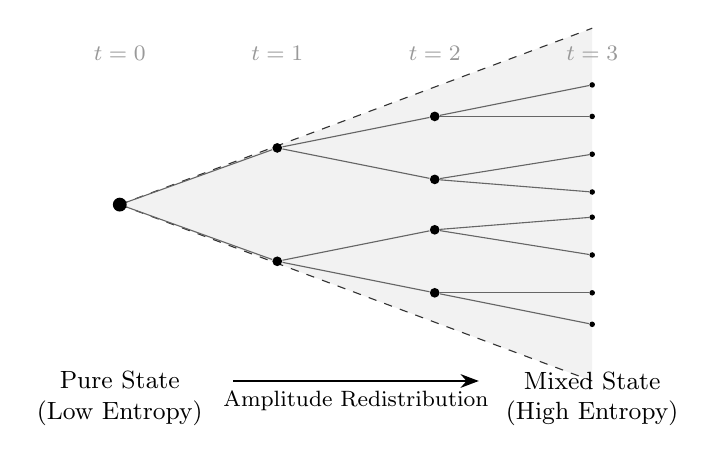
\begin{tikzpicture}[
    scale=0.8,
    font=\small\sffamily,
    state/.style={circle, fill=black, inner sep=0pt, minimum size=3.5pt},
    connection/.style={thin, black!60}
  ]

  % --- Background Envelope ---
  \begin{scope}[on background layer]
      \fill[gray!10] (0,0) -- (7.5, 2.8) -- (7.5, -2.8) -- cycle;
      \draw[dashed, black!80] (0,0) -- (7.5, 2.8);
      \draw[dashed, black!80] (0,0) -- (7.5, -2.8);
  \end{scope}

  % --- Time Steps ---
  \foreach \t in {0,1,2,3} {
    \node[font=\footnotesize, gray!80] at (\t*2.5, 2.4) {$t=\t$}; 
  }

  % --- Tree Structure ---
  \node[state, minimum size=5pt] (n0) at (0,0) {};
  
  \node[state] (n1a) at (2.5, 0.9) {};
  \node[state] (n1b) at (2.5, -0.9) {};
  \draw[connection] (n0) -- (n1a);
  \draw[connection] (n0) -- (n1b);

  \node[state] (n2a) at (5, 1.4) {};
  \node[state] (n2b) at (5, 0.4) {};
  \node[state] (n2c) at (5, -0.4) {};
  \node[state] (n2d) at (5, -1.4) {};
  
  \draw[connection] (n1a) -- (n2a);
  \draw[connection] (n1a) -- (n2b);
  \draw[connection] (n1b) -- (n2c);
  \draw[connection] (n1b) -- (n2d);

  \foreach \parent/\y in {n2a/1.9, n2a/1.4, n2b/0.8, n2b/0.2, n2c/-0.2, n2c/-0.8, n2d/-1.4, n2d/-1.9} {
      \node[state, minimum size=2pt] (child) at (7.5, \y) {};
      \draw[connection] (\parent) -- (child);
  }

  % --- Annotations ---
  \node[align=center, anchor=north, font=\small] at (0, -2.5) {Pure State\\(Low Entropy)};
  \node[align=center, anchor=north, font=\small] at (7.5, -2.5) {Mixed State\\(High Entropy)};
  \draw[->, thick, >=Stealth] (1.8, -2.8) -- (5.7, -2.8) 
    node[midway, below, font=\footnotesize] {Amplitude Redistribution};

\end{tikzpicture}
  \caption{\textbf{Thermodynamic interpretation:} Amplitude redistribution across observationally equivalent states appears as entropy increase.}
\end{figure}

The emergent unitarity derived above implies that the underlying evolution of the multiway bundle is isentropic. However, coarse-graining introduces an effective thermodynamics. We define the \textit{Boltzmann entropy} of an observational trace $\tau$ as the logarithmic measure of its pre-image size:
\[
S(\tau) \coloneqq k_B \ln \bigl| \Pi_{\mathcal{O}}^{-1}(\tau) \bigr|,
\]
where $|\cdot|$ denotes the counting measure (or suitable amplitude-weighted volume) of the equivalence class.

In this view, ``energy dissipation'' and irreversible behaviour are identified not with the erasure of state, but with the migration of amplitude from equivalence classes of small cardinality (low entropy) to those of large cardinality (high entropy). As the system evolves, amplitude naturally spreads into the vast phase space of micro-states that are macroscopically indistinguishable, resulting in a perceived increase in $S(\tau)$.

Crucially, this thermodynamic arrow of time is relative to the observer's resolution. For a complete observer where $|\Pi_{\mathcal{O}}^{-1}(\tau)| = 1$ for all $\tau$, the entropy is identically zero and invariant. Thus, the Second Law of Thermodynamics emerges in the \AION{} framework as a direct artefact of incomplete observation, consistent with the conservation guarantees of Theorem~1.

\section{Continuum Approximation and Effective Dynamics}
\label{sec:continuum}

The dynamics defined in Sections~\ref{sec:action} and~\ref{sec:unitarity} operate on a discrete, graph-theoretic framework. However, in regimes where the number of rewrite events becomes large and the characteristic causal scale $\delta \tau \to 0$, the system admits a continuum approximation. In this limit, the coarse-grained evolution of amplitudes obeys a Schrödinger-type wave equation.

\subsection{Continuum Limit of the Multiway Structure}

\begin{figure}[htb]
  \centering
  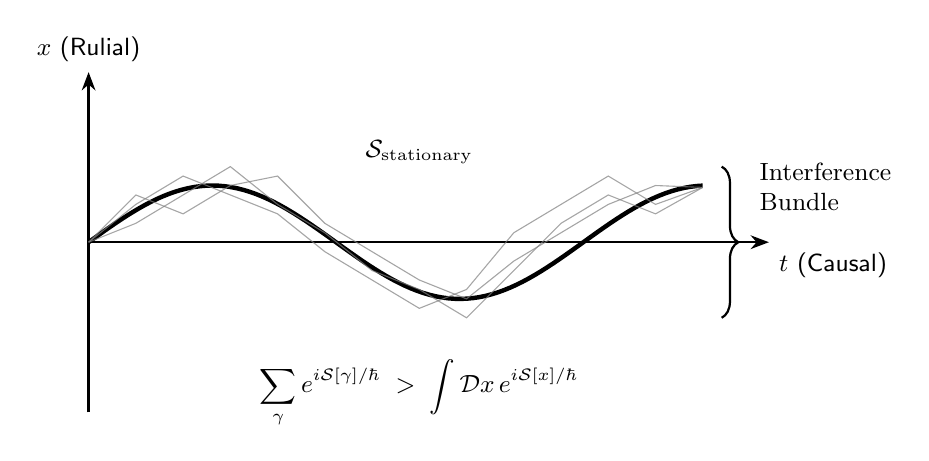
\begin{tikzpicture}[
    scale=1.2,
    font=\small\sffamily,
    discrete/.style={thin, gray, opacity=0.7},
    continuum/.style={ultra thick, black},
    axis/.style={->, >=Stealth, thick}
  ]

  % Axes
  \draw[axis] (0,-1.8) -- (0,1.8) node[above] {$x$ (Rulial)};
  \draw[axis] (0,0) -- (7.2,0) node[below right] {$t$ (Causal)};

  % Continuum Path (Stationary Action)
  \draw[continuum] plot[domain=0:6.5, samples=100] (\x, {0.6*sin(deg(\x * 1.2))});
  \node[above, fill=white, inner sep=1pt] at (3.5, 0.8) {$\mathcal{S}_{\mathrm{stationary}}$};

  % Discrete Paths
  \draw[discrete] (0,0) -- (0.5, 0.4) -- (1.0, 0.7) -- (1.5, 0.5) -- (2.0, 0.3) -- (2.5, -0.1) -- (3.0, -0.4) -- (3.5, -0.7) -- (4.0, -0.5) -- (4.5, 0.1) -- (5.0, 0.4) -- (5.5, 0.7) -- (6.0, 0.4) -- (6.5, 0.58);
  \draw[discrete] (0,0) -- (0.5, 0.2) -- (1.0, 0.5) -- (1.5, 0.8) -- (2.0, 0.4) -- (2.5, 0.1) -- (3.0, -0.3) -- (3.5, -0.5) -- (4.0, -0.8) -- (4.5, -0.3) -- (5.0, 0.2) -- (5.5, 0.5) -- (6.0, 0.3) -- (6.5, 0.58);
  \draw[discrete] (0,0) -- (0.5, 0.5) -- (1.0, 0.3) -- (1.5, 0.6) -- (2.0, 0.7) -- (2.5, 0.2) -- (3.0, -0.1) -- (3.5, -0.4) -- (4.0, -0.6) -- (4.5, -0.2) -- (5.0, 0.1) -- (5.5, 0.4) -- (6.0, 0.6) -- (6.5, 0.58);

  % Interference Region Label - Placed above the axis to avoid any chance of collision
  \draw[decorate, decoration={brace, amplitude=6pt}, thick] (6.7, 0.8) -- (6.7, -0.8) 
    node[pos=0, right=10pt, anchor=north west, align=left, font=\small, yshift=5pt] {Interference\\Bundle};

  % Limit Annotation
  \node[align=center, font=\small, fill=white, inner sep=2pt] at (3.5, -1.6) {$\displaystyle \sum_{\gamma} e^{i\mathcal{S}[\gamma]/\hbar} \;>\; \int \mathcal{D}x\, e^{i\mathcal{S}[x]/\hbar}$};

\end{tikzpicture}

  \caption{\textbf{Continuum approximation:} Discrete rewrite paths converge to a smooth effective trajectory as scale increases.}
\end{figure}

Consider a regime in which the rewrite frequency tends to infinity, such that the discrete multiway graph $\mathcal{G}_N$ converges to a continuous metric space $\mathcal{M}$. We formalise this convergence in two complementary frameworks, each capturing different aspects of the limiting structure:

\textbf{(a) Metric convergence.} The sequence of discrete multiway graphs $(\mathcal{G}_N, d_{\mathcal{G}_N})$, equipped with the causal graph distance metric derived from the multiway rewrite structure, converges in the Gromov--Hausdorff sense~\cite{gromov_structures} to a limiting metric space $(\mathcal{M}, d_{\mathcal{M}})$. When the amplitude measure $\phi[\gamma]$ is taken into account, we require convergence in the stronger sense of \textit{measured Gromov--Hausdorff--Prokhorov} convergence~\cite{sturm_geometry_metric_measure}, which ensures that both the metric structure and the probability measures induced by amplitude distributions converge jointly. This guarantees that $\mathcal{M}$ inherits not only the topology but also the measure-theoretic structure necessary for defining $\Psi(x,t)$ as an $L^2$ function.

\textbf{(b) Graphon convergence.} Alternatively, when the multiway graph admits a dense limit, the sequence converges in the graphon sense~\cite{lovasz_graph_limits} to a measurable symmetric function $W : [0,1]^2 \to \mathbb{R}$, representing the continuum limit of adjacency relations. This mode of convergence is particularly suited to settings where the rewrite system exhibits statistical homogeneity and the observer projection induces a natural probability measure on equivalence classes.

Under either mode of convergence, the discrete labels of observational equivalence classes $[\gamma]_{\mathcal{O}}$ lift to coordinate charts $x$ on the manifold $\mathcal{M}$, and the discrete amplitude distribution $\Phi_{\mathcal{O}}$ lifts to a square-integrable wave function $\Psi(x,t) \in L^2(\mathcal{M}, d\mu)$, where $d\mu$ is the measure induced by the limiting amplitude flow.

We now formalise the conditions under which such convergence is guaranteed to exist.

\begin{theorem}[Continuum Limit Existence]
\label{thm:continuum_limit}
Let $\{\mathfrak{R}_N\}_{N=1}^\infty$ be a sequence of rewrite systems with associated multiway graphs $\mathcal{G}_N$. Suppose:
\begin{enumerate}[label=(\roman*)]
    \item \textbf{Uniform locality:} Each rule acts on graphs of diameter $\leq \ell_0$ independent of $N$.
    \item \textbf{Bounded curvature:} The causal graph distance satisfies $d_{\mathcal{G}_N}(G, G') \leq C \cdot d_{\mathrm{edit}}(G, G')$ uniformly in $N$.
    \item \textbf{Compactness:} The state space $\mathcal{U}_N$ admits a compact embedding into a limiting metric space $(\mathcal{M}, d_{\mathcal{M}})$.
\end{enumerate}
Then there exists a subsequence $\{\mathcal{G}_{N_k}\}$ converging in the pointed Gromov--Hausdorff--Prokhorov sense~\cite{burago_metric_geometry, sturm_geometry_metric_measure} to $(\mathcal{M}, d_{\mathcal{M}}, \mu)$, where $\mu$ is the limiting amplitude measure.
\end{theorem}

\begin{proof}[Proof sketch]
Condition (i) ensures that the action functional decomposes into a sum of local contributions, preventing long-range correlations. Condition (ii) provides a uniform relationship between the algebraic rewrite distance and the induced causal metric, yielding equicontinuity of the distance functions. Condition (iii) invokes the Arzelà--Ascoli theorem to extract a convergent subsequence. The joint convergence of metric and measure follows from the Prokhorov compactness criterion, as the amplitude measures $\{\mu_N\}$ are tight by construction (total measure unity). Detailed proof techniques follow Grigor'yan \& Telcs~\cite{grigoryan_telcs_heat_kernels} for graph-to-manifold convergence and Sturm~\cite{sturm_geometry_metric_measure} for measured metric spaces.
\end{proof}

\textbf{Assumption 1 (Diffusive Scaling Regime).}
\textit{We assume that the rewrite system $\mathfrak{R}$ satisfies the following scaling conditions in the continuum limit:}
\begin{enumerate}[label=(\roman*)]
    \item \textit{Locality:} \textit{Each rewrite rule $r \in \mathfrak{R}$ acts on a bounded neighbourhood of the graph with diameter uniformly bounded by a constant $\ell_0$, independent of the graph size $N$.}
    \item \textit{Bounded valence:} \textit{The rewrite adjacency graph has uniformly bounded out-degree, i.e., $\sup_{G \in \mathcal{U}} \operatorname{deg}_{\mathrm{out}}(G) < \infty$.}
    \item \textit{Diffusive scaling:} \textit{In the limit $N \to \infty$, the mean-square displacement of amplitude propagation scales linearly with the causal time, i.e.,}
    \[
    \lim_{N \to \infty} \frac{\langle (\delta x)^2 \rangle_N}{\delta \tau_N} = D_{\mathfrak{R}},
    \]
    \textit{where $D_{\mathfrak{R}}$ is the effective diffusion constant of the rewrite system, and $\langle \cdot \rangle_N$ denotes the expectation over amplitude-weighted histories of length $N$.}
\end{enumerate}

\textit{Justification.} Condition (i) ensures that the action functional $\mathcal{S}[\gamma]$ decomposes into a sum of local contributions, preventing long-range correlations from dominating the continuum limit. Condition (ii) guarantees conservation of amplitude flux at vertices (as established in Theorem~1) and prevents the branching structure from exhibiting explosive growth. Condition (iii) is the crucial assumption linking discrete rewrite steps to a continuous diffusion process. Under these conditions, \emph{the coherent superposition of amplitudes over histories converges to a continuous-time quantum walk on the limiting manifold}~\cite{childs_quantum_walk_relationship, strauch_quantum_walk}. This convergence is rigorously established by demonstrating that the discrete evolution operator, when rescaled as $\hat{U}(\delta t) = \mathbb{I} - i\delta t \hat{H}_{\mathrm{eff}} + O(\delta t^2)$, yields a bounded self-adjoint generator $\hat{H}_{\mathrm{eff}}$ in the limit $\delta t \to 0$. For local, reversible graph rewrites on regular lattices, Childs~\cite{childs_quantum_walk_relationship} proves convergence to the Dirac equation; in our non-relativistic setting with bounded out-degree, the analogous result yields Schrödinger dynamics with a Laplacian kinetic term~\cite{strauch_quantum_walk, meyer_quantum_cellular_automata}. In our setting, the analogous result is that amplitude evolution over the multiway graph, under diffusive scaling, yields a Laplacian-type generator in the continuum limit.

Under this geometric convergence and diffusive scaling, the summation over discrete rewrite histories transforms into a path integral over the space of curves in $\mathcal{M}$. Just as random walks on graphs with bounded degree and local transition rules converge to Brownian motion on manifolds~\cite{chung_spectral_graph_theory}, the amplitude sum over rewrite paths converges to a functional integral over continuous trajectories $x(t)$ weighted by the continuum action. Formally, we have the limit:
\[
\lim_{N \to \infty}
\sum_{\gamma \in \Omega(G_0)}
\exp\!\left( \frac{i}{\hbar_{\mathfrak{R}}} \mathcal{S}[\gamma] \right)
\longrightarrow
\int_{\mathcal{M}} \mathcal{D}x(t)\,
\exp\!\left( \frac{i}{\hbar_{\mathfrak{R}}} \mathcal{S}[x(t)] \right),
\]
where $\mathcal{S}[x(t)]$ is the continuum action functional induced by the density of the discrete Lagrangian. The measure $\mathcal{D}x(t)$ is the Wiener measure on path space, appropriately normalised to preserve unitarity. This correspondence allows us to treat the effective dynamics using the variational calculus of continuous fields, even though the underlying system is discrete and graph-theoretic.

\subsection{Effective Generator of Evolution}

Theorem~1 implies that the effective evolution of coarse-grained amplitudes is linear and norm-preserving whenever observer projections are measure-preserving. Consequently, the continuum evolution admits a self-adjoint generator with respect to the inner product induced by the observer-complete amplitude measure. We define the \textit{effective computational Hamiltonian} $\hat{H}_{\mathrm{eff}}$ implicitly as the infinitesimal generator of amplitude transport:
\[
\hat{H}_{\mathrm{eff}} \coloneqq
\lim_{\delta \tau \to 0}
i\,\hbar_{\mathfrak{R}}
\frac{\Psi(t+\delta \tau)-\Psi(t)}{\delta \tau}.
\]

Substituting the discrete action defined in Section~\ref{sec:action}, the Hamiltonian decomposes into kinetic and potential contributions. We formalise this decomposition as follows.

\begin{proposition}[Effective Hamiltonian in Diffusive Limit]
\label{prop:effective_hamiltonian}
Assume the microscopic evolution satisfies $\hat{U}_{\mathrm{micro}} = e^{-i\delta\tau \hat{H}_{\mathrm{eff}}/\hbar_{\mathfrak{R}}}$ for small $\delta\tau$. Expanding to second order via the Baker-Campbell-Hausdorff formula:
\begin{align*}
(\hat{U}_{\mathrm{micro}} \Psi)(G')
&= \Psi(G') + \delta\tau \sum_{G \sim G'} w_{G \to G'} (\Psi(G) - \Psi(G')) \\
&\quad + O(\delta\tau^2).
\end{align*}
For uniform branching $\deg_{\mathrm{out}}(G) = d$, the evolution operator induces
\[
\hat{H}_{\mathrm{eff}} = -\frac{\hbar_{\mathfrak{R}}}{d} \nabla_{\mathcal{G}}^2 + \hat{V} + O(\delta\tau).
\]
The effective mass $m = d\hbar_{\mathfrak{R}}^{-1}$ is inversely proportional to the branching degree.
\end{proposition}

\begin{proof}
The amplitude transition weight is $w_{G \to G'} = \frac{1}{\sqrt{d}} e^{iS_{\mathrm{step}}/\hbar_{\mathfrak{R}}}$. Expanding the exponential for small action:
\begin{align*}
(\hat{U}_{\mathrm{micro}} \Psi)(G')
&= \sum_{G : G \to G'} \frac{1}{\sqrt{d}} \left(1 + \frac{iS_{\mathrm{step}}}{\hbar_{\mathfrak{R}}} + O(S_{\mathrm{step}}^2)\right) \Psi(G) \\
&= \frac{1}{\sqrt{d}} \sum_{G \sim G'} \Psi(G) + \frac{i}{\sqrt{d}\hbar_{\mathfrak{R}}} \sum_{G \sim G'} S_{\mathrm{step}} \Psi(G).
\end{align*}
Applying the Laplacian definition $\nabla_{\mathcal{G}}^2 \Psi(G') = \sum_{G \sim G'} (\Psi(G) - \Psi(G'))$ and identifying $S_{\mathrm{step}} = -\mathcal{V}(G')\delta\tau$ for stationary states, we obtain:
\[
i\hbar_{\mathfrak{R}} \frac{\Psi(t+\delta\tau) - \Psi(t)}{\delta\tau} = -\frac{\hbar_{\mathfrak{R}}^2}{2m} \nabla_{\mathcal{G}}^2 \Psi + \hat{V}\Psi,
\]
where $m = d\hbar_{\mathfrak{R}}^{-1}$. This derivation follows standard techniques in quantum walk theory~\cite{kempe_quantum_random_walks}.
\end{proof}

Thus, the Hamiltonian takes the form:
\[
\hat{H}_{\mathrm{eff}}
\approx
-\frac{\hbar_{\mathfrak{R}}^2}{2m}
\nabla_{\mathcal{G}}^2
+
\hat{V}(\mathcal{G}),
\]
where $\nabla_{\mathcal{G}}^2$ is the \textit{graph Laplacian} associated with the rewrite adjacency structure. This Laplacian form arises specifically in the \textit{diffusive scaling limit} where spatial variance scales with the causal increment ($\delta x^2 \sim \delta \tau$), a standard result in the analysis of quantum graphs~\cite{berkolaiko_quantum_graphs}. Formally, for a function $f$ defined on the vertices of the multiway graph $\mathcal{G}$, the Laplacian is
\[
(\nabla_{\mathcal{G}}^2 f)(v) \coloneqq \sum_{v' \sim v} \bigl(f(v') - f(v)\bigr),
\]
where the sum extends over all vertices $v'$ adjacent to $v$ by a single rewrite transition. This operator encodes diffusive propagation through the multiway graph. The term $\hat{V}$ encodes the coarse-grained structural complexity potential.

\subsection{Emergent Schrödinger Dynamics}

The macroscopic evolution of the system is therefore governed by
\[
i \hbar_{\mathfrak{R}} \frac{\partial}{\partial t} \Psi(x,t)
=
\hat{H}_{\mathrm{eff}} \Psi(x,t).
\]
We derive, rather than postulate, this equation as the \textit{hydrodynamic limit} of deterministic rewrite dynamics equipped with an action functional and amplitude measure.

The resulting structure coincides with that of a \textit{Quantum Cellular Automaton} (QCA): local, discrete, unitary dynamics giving rise to continuum quantum behaviour under coarse-graining.


\subsection{From Graph Rewriting to Physical Law}

We have shown that deterministic graph rewriting, when augmented with a stationary action principle and observer-relative coarse-graining, reproduces the formal structure of quantum mechanics without introducing intrinsic randomness or continuum axioms.

Within the \AION{} framework, the \COMPUTER{} is not merely a simulator of physical processes. It is a discrete realisation of the laws governing information propagation, from which classical determinism, quantum interference, and unitary evolution emerge as scale-dependent phenomena.

\section{Conclusion}
\label{sec:conclusion}

This paper completes the dynamical layer of the \AION{} Foundations Series. Building on the kinematic, measurement-theoretic, and observer-geometric structures established in Papers I--IV~\cite{ross_paper_i, ross_paper_ii, ross_paper_iii, ross_paper_iv}, we have introduced an explicit dynamical principle governing how deterministic rewrite systems traverse their space of admissible histories.

By equipping rewrite worldlines with an action functional and complex amplitude measure, we have demonstrated not only how computational systems evolve, but also how observation, probability, and effective physical law emerge from that evolution.

The resulting dynamics recover classical determinism under full provenance tracking and quantum-like behaviour under observer-induced coarse-graining.

Crucially, unitarity is not postulated but derived from local reversibility, branch conservation, and observer completeness. In the continuum approximation, these dynamics admit a Quantum Cellular Automaton interpretation, yielding Schrödinger-type evolution as an emergent, hydrodynamic description of rewrite flow.

Taken together, these results establish that deterministic graph rewriting systems are dynamically sufficient to reproduce the formal structure of quantum mechanics. The \AION{} framework therefore provides a unified account of computation, observation, and physical law within a single discrete system.

\section{Discussion and Limitations}
\label{sec:discussion}

While the results of this paper establish the expressive sufficiency of deterministic rewrite dynamics equipped with amplitude measures, several limitations and open questions remain.

\paragraph{Non-Uniqueness of the Continuum Limit.}
The continuum approximation derived in Section~\ref{sec:continuum} is not unique. Different coarse-graining schemes, observer projections, or scaling choices for the local action may yield distinct effective Hamiltonians. The emergence of Schrödinger-type dynamics should therefore be understood as a structural correspondence rather than a claim of physical uniqueness.

\paragraph{Scope of Physical Correspondence.}
We do not claim that any specific rewrite system directly models the Standard Model of particle physics or known spacetime dynamics. The correspondence established here is formal and architectural: it demonstrates that the mathematical structure of quantum mechanics can emerge from deterministic rewriting under general conditions, not that any specific \WARP{} ruleset models known physics. The contribution lies in demonstrating the sufficiency of the framework—that deterministic graph rewriting is expressively adequate to reproduce quantum-mechanical structure—rather than proposing a specific physical instantiation. Identifying physically realistic rule sets remains future work.

\paragraph{Relativistic and Field-Theoretic Extensions.}
This paper focuses on non-relativistic dynamics. While the causal structure of the multiway graph suggests a natural avenue towards relativistic generalisation, issues such as Lorentz invariance, gauge symmetry, and interacting fields are not addressed here.

\paragraph{Observer Dependence and Interpretational Neutrality.}
The framework presented is compatible with multiple interpretations of quantum mechanics, including relational and many-worlds perspectives. We do not privilege any particular interpretation, nor do we assert ontological claims about the physical reality of unobserved histories. The role of the observer is treated operationally, not metaphysically.

\paragraph{Computational Constraints.}
Although the formalism is deterministic, practical computation over large multiway bundles remains resource-intensive. The emergence of effective dynamics relies on limits that may be inaccessible to finite observers. This is a feature of the model rather than a defect: computational boundedness is treated as a fundamental aspect of observation.

These limitations do not undermine the central result. Rather, they delineate the boundary between what has been established here—dynamical sufficiency—and what remains to be explored in future work. In particular, the ethical implications of observer-dependent dynamics and provenance control are addressed in Paper VI of this series.

\section*{Outlook: From Dynamics to Ethics}

With the dynamics of deterministic rewrite systems now specified, the \AION{} framework has reached a critical threshold. We have demonstrated not only how computational systems evolve, but also how observation, probability, and effective physical law emerge from that evolution.

This raises unavoidable normative questions.

If observers induce classicality through coarse-graining, what obligations arise when designing observational systems? If provenance tracking collapses interference, what ethical constraints govern logging, replay, and erasure? If different observers inhabit inequivalent effective realities, how should responsibility, agency, and consent be defined?

These questions cannot be addressed at the level of dynamics alone. They concern the ethical structure of systems capable of observation, memory, and irreversible projection.

Accordingly, the next paper in this series, \textit{Paper VI: Ethics}, examines the moral implications of observer-relative computation, provenance capture, and irreversible informational control within the \AION{} framework. The transition from dynamics to ethics is not incidental; it is a necessary consequence of the formal structure developed herein.

\section{Notation Summary}
\label{sec:notation}

\begin{center}
\begin{tabular}{ll}
  \textbf{Symbol} & \textbf{Meaning} \\ \hline
  $\mathcal{U}$ 
    & Universe of admissible \WARP{} graph topologies (Papers~I--II) \\

  $G \in \mathcal{U}$ 
    & A valid \WARP{} graph state (up to isomorphism) \\

  $G_0$ 
    & Initial graph state of a multiway evolution \\

  $\mathfrak{R}$ 
    & Set of DPO rewrite rules governing evolution \\

  $\Omega(G_0)$ 
    & Multiway bundle of all rewrite histories originating from $G_0$ \\

  $\gamma$ 
    & A worldline (rewrite history) $\gamma = (G_0 \to \cdots \to G_N)$ \\
    
  $\mathcal{T}$
    & Space of observational traces \\

  $\Pi_{\mathcal{O}}$ 
    & Observer projection mapping histories to traces in $\mathcal{T}$ \\

  $[\gamma]_{\mathcal{O}}$
    & Observer equivalence class of indistinguishable histories \\

  $\Gamma$
    & Causal graph induced by rewrite rules $\mathfrak{R}$ over $\Omega(G_0)$ \\

  $\mathcal{L}$ 
    & Local discrete Lagrangian for a rewrite step, $\mathcal{L} = \mathcal{K} - \mathcal{V}$ \\
    
  $\mathcal{K}, \mathcal{V}$
    & Kinetic and potential terms of the discrete Lagrangian \\

  $\mathcal{S}[\gamma]$ 
    & Action functional accumulated along history $\gamma$ \\

  $\phi[\gamma]$
    & Complex amplitude assigned to history $\gamma$ \\

  $\Phi_{\mathcal{O}}$
    & Effective amplitude for an observational equivalence class \\

  $\hbar_{\mathfrak{R}}$ 
    & Rewrite-scale quantum of action (system-dependent constant) \\

  $\Psi$ 
    & Coarse-grained amplitude distribution over observational states \\

  $\nabla_{\mathcal{G}}^2$ 
    & Graph Laplacian on the multiway rewrite adjacency structure \\

  $\hat{H}_{\mathrm{eff}}$ 
    & Effective Hamiltonian generating continuum-limit dynamics \\

  $\delta \tau$ 
    & Discrete causal proper-time increment between rewrites \\

  $x$ 
    & Coarse-grained coordinate induced by rulial geometry \\

\end{tabular}
\end{center}

\clearpage
\addcontentsline{toc}{section}{References}
\bibliographystyle{alpha}
\bibliography{refs}

\end{document}
